\section{Redux} 
\subsection{Overview}
Redux\glosp is a \texttt{npm} module which manage the entire state of the website from client-side. It consists of:
\begin{itemize}
	\item Actions;
	\item Reducers;
	\item Store.
\end{itemize}
When the website is built, a default state for the store is set (it is defined into the reducer JavaScript file).
\subsection{Unidirectional pattern} 
Basically some actions are mapped by \texttt{container components} into specific \texttt{presentational components} through them props with \texttt{Connect(arg1, arg2)} method. When a presentational component request a \texttt{dispatch()} of a specific action, a reducer will complete the request by changing the store and returning a new instance of the application state. Each time the store is changed, the \texttt{Render()} method of displayed components is called.
\texttt{Redux} is the name of the pattern implemented by React and Redux, it is an evolution of \texttt{Flux} pattern, the difference is that Flux uses more than one store.\\
\begin{figure}[H]
	\centering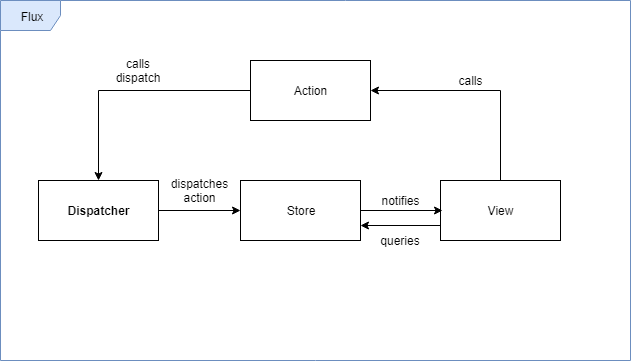
\includegraphics[scale = 0.6]{res/images/Flux.png}
	\caption{Flux pattern}
\end{figure}

\subsection{Actions}
There are twelve different actions inside the \texttt{src/actions/} folder. Each action is called by the \texttt{action creator} when a container component request it's dispatch. Here there is the list of actions and what them do when they are invoked.
\begin{itemize}
	\item \textbf{ACLogin}: it changes the \texttt{logged} state value;
	\item \textbf{ACIncreaseQuantity}: it increases the quantity of a product that is inside the cart, by changing the \texttt{quantity} value of a specified product inside \texttt{cart} state value;
	\item \textbf{ACCartToOrders}: it copies all the content of \texttt{cart} state value to \texttt{ordersList} state value, finally it resets the \texttt{cart} state value;
	\item \textbf{ACSignUp}: it provides to save into the store all of the user informations after they are successfully saved into IPFS\glo;
	\item \textbf{ACAddToCart}: it puts the selected product with selected quantity into \texttt{cart} state value;
	\item \textbf{ACSearch}: it changes \texttt{searchProduct} state value for making a dynamic search inside store page;
	\item \textbf{ACLogout}: it changes the \texttt{logged} state value;
	\item \textbf{ACAddToSelling}: it puts the product into \texttt{selling} state value after it is successfully saved into IPFS;
	\item \textbf{ACReset}: it resets the entire state of application, even if \texttt{redux-persist} is present;
	\item \textbf{ACRemoveFromCart}: it removes the selected product from \texttt{cart} state value;
	\item \textbf{ACDecreaseQuantity}: it decreases the quantity of a product that is inside the cart, by changing the \texttt{quantity} value of a specified product inside \texttt{cart} state value;
	\item \textbf{ACDisableAccount}: it sets a value different from 0 to \texttt{error} state value if something goes wrong, otherwise it sets 0 into \texttt{error} state value.
\end{itemize}
\subsection{Reducers}
\begin{itemize}
	\item \textbf{ReducerAuth}: it makes the dispatch of the actions inside:
	\begin{itemize}
		\item ACLogin;
		\item ACLogout;
		\item ACSignUp;
		\item ACReset.
	\end{itemize}
	\item \textbf{ReducerSearch}: it makes the dispatch of search action;
	\item \textbf{ReducerCart}: it makes the dispatch of the actions inside:
	\begin{itemize}
		\item ACIncreaseQuantity;
		\item ACDecreaseQuantity;
		\item ACCartToOrders;
		\item ACAddToCart;
		\item ACAddToSelling;
		\item ACRemoveFromCart.
	\end{itemize}
	\item \textbf{ReducerGovernment}: it makes the dispatch of disableAccount action.
\end{itemize}
\subsection{Store}
It's configuration resides into root reducer file, the initial configuration is:
\begin{itemize}
	\item logged: false;
	\item user: null;
	\item searchProduct: "";
	\item cart: [ ];
	\item pending: [ ];
	\item ordersList: [ ];
	\item error: 0.
\end{itemize}
Each time the \texttt{reset} action is dispatched from it's reducer, the initial configuration of the store is set.

\subsection{Redux-Persist}
It is a \texttt{npm} module used for maintaining the current store even if the user leaves the website. It is browser-locally saved, so if a user will enter into the website from another device or from another browser, the store will be set with default values. It has a blacklist for bypassing some values, in this way reloading the website, these values will not be saved (the blacklist is defined into reducer JavaScript file).

\begin{landscape}
	\subsection{UML} 
	
	\begin{figure}[H]
		\centering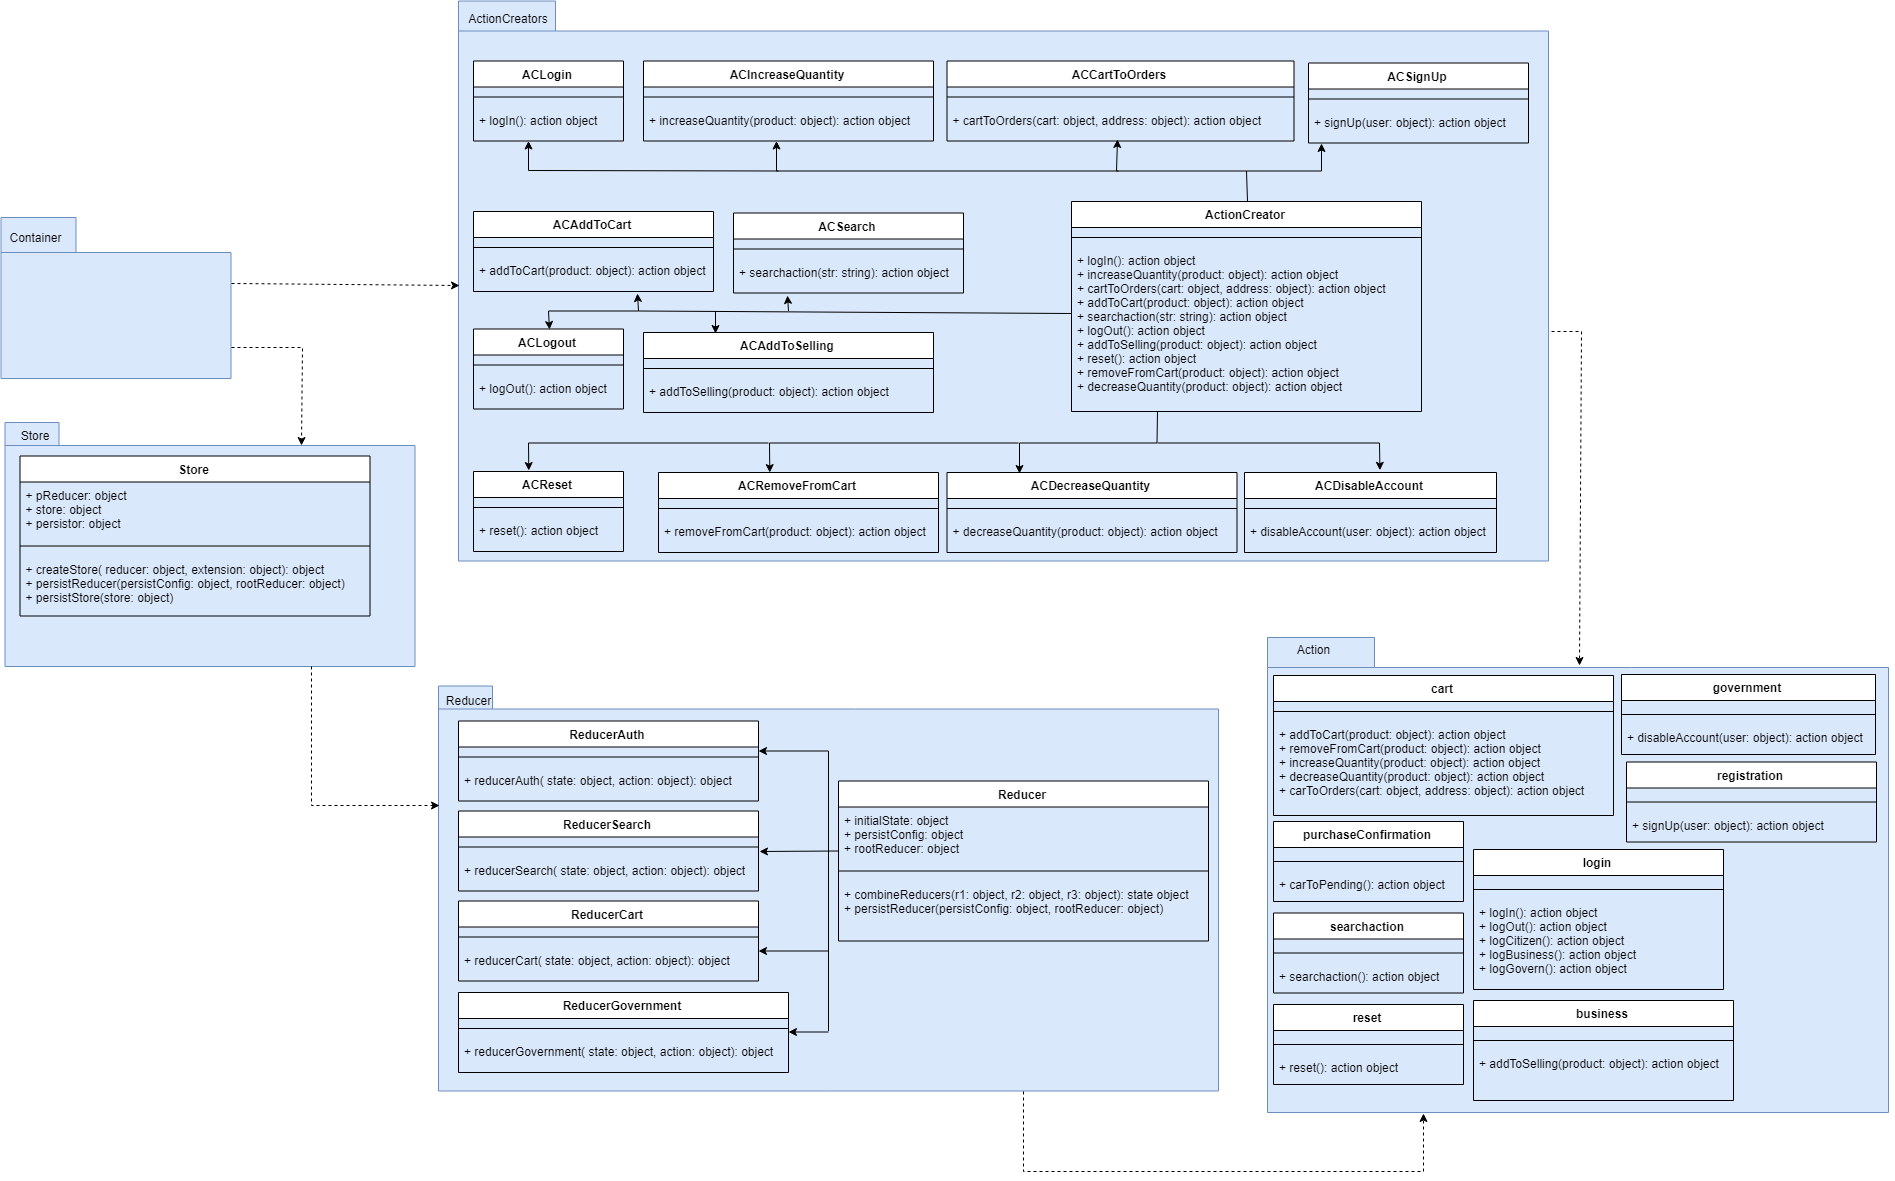
\includegraphics[scale = 0.3]{res/images/ReduxDiagram.png}
		\caption{Redux architecture}
	\end{figure}
\end{landscape}